%%%%%%%%%%%%%%%%%%%%%%%%%%%%%%%%%%%%%%%%%
% Beamer Presentation
% LaTeX Template
% Version 1.0 (10/11/12)
%
% This template has been downloaded from:
% http://www.LaTeXTemplates.com
%
% License:
% CC BY-NC-SA 3.0 (http://creativecommons.org/licenses/by-nc-sa/3.0/)
%
%%%%%%%%%%%%%%%%%%%%%%%%%%%%%%%%%%%%%%%%%

\documentclass{beamer}

\mode<presentation> {

\usetheme{Madrid}

\setbeamertemplate{navigation symbols}{} % Remove the navigation symbols from the bottom of all slides
}

\usepackage{chronology}
\usepackage{graphicx} % Allows including images
\usepackage{listings} % Allows including code
\usepackage{color}

\definecolor{dkgreen}{rgb}{0,0.6,0}
\definecolor{gray}{rgb}{0.5,0.5,0.5}
\definecolor{mauve}{rgb}{0.58,0,0.82}
\definecolor{links}{HTML}{2A1B81}
\hypersetup{colorlinks,linkcolor=,urlcolor=links}

\graphicspath{ {./images/} }

% Insert code
% https://stackoverflow.com/questions/3175105/inserting-code-in-this-latex-document-with-indentation
\lstset{frame=tb,
  language=Java,
  showstringspaces=false,
  columns=flexible,
  basicstyle={\small\ttfamily},
  keywordstyle=\color{blue},
  commentstyle=\color{dkgreen},
  stringstyle=\color{mauve},
  breaklines=true
}

%----------------------------------------------------------------------------------------
% TITLE PAGE
%----------------------------------------------------------------------------------------

\title[Rust]{Rust} % The short title appears at the bottom of every slide, the full title is only on the title page
\author{Carlos A. Molina}
\date{May 18, 2022}

\begin{document}

\begin{frame}
\titlepage % Print the title page as the first slide
\end{frame}

\begin{frame}
\frametitle{Table of contents}
\tableofcontents % Throughout your presentation, if you choose to use \section{} and \subsection{} commands, these will automatically be printed on this slide as an overview of your presentation
\end{frame}

%----------------------------------------------------------------------------------------
% PRESENTATION SLIDES
%----------------------------------------------------------------------------------------

%------------------------------------------------
\section{Introduction} % Sections can be created in order to organize your presentation into discrete blocks, all sections and subsections are automatically printed in the table of contents as an overview of the talk
%------------------------------------------------

\begin{frame}

\frametitle{Logo and mascot}

\begin{columns}[c] % The "c" option specifies centered vertical alignment while the "t" option is used for top vertical alignment

\column{.45\textwidth}

  \begin{figure}
    \centering
    \href{https://foundation.rust-lang.org/img/rust-logo-blk.svg}
      {
\includegraphics[width=0.5\textwidth]{rust-logo-blk.png}}
    \caption{Rust logo}
  \end{figure}

\column{.5\textwidth}
  \begin{figure}
    \centering
    \href{https://rustacean.net/assets/rustacean-orig-noshadow.svg}
      {
\includegraphics[width=0.5\textwidth]{rustacean-orig-noshadow.png}}
    \caption{Ferris the crab. Unofficial mascot}
  \end{figure}

\end{columns}

\end{frame}

\begin{frame}
\frametitle{History}

\begin{chronology}[5]{2004}{2021}{\textwidth}
    \event{2006}{Personal project}
    \event{2009}{Mozilla sponsoring}
    \event{2010}{First appearing}
    \event{2012}{Pre-alpha release}
    \event{2015}{Rust 1.0}
    \event{2020}{COVID-19 layoffs}
    \event{2021}{Rust Foundation}
\end{chronology}

\begin{columns}[c] % The "c" option specifies centered vertical alignment while the "t" option is used for top vertical alignment

\column{.3\textwidth}

  \begin{figure}
    \centering
    \href{https://github.com/graydon}
      {
\includegraphics[width=0.35\textwidth]{graydon-github.png}}
    \caption{Graydon Hoare}
  \end{figure}

\column{.7\textwidth}
  \begin{figure}
    \centering
    \href{https://foundation.rust-lang.org/members/}
      {
\includegraphics[width=0.5\textwidth]{rust-foundation-founding-members.png}}
    \caption{Rust Foundation founding members}
  \end{figure}

\end{columns}

\end{frame}

\section{Features}

\begin{frame}
\frametitle{Features}

\begin{itemize}
\item Low-level
\item Compiled
\item Performance: no garbage collector
\item Type system and ownership model guarantee:
  \begin{itemize}
  \item Memory-safety
  \item Thread-safety
  \end{itemize}
\item Cargo: cargo build, cargo fmt...
\item Crates: \href{https://crates.io/}{crates.io}
\end{itemize}

\end{frame}

\begin{frame}[fragile]
\frametitle{Features. Ownership}

\begin{lstlisting}
fn main() {
    let mut tribe_name = String::from("Backend"); // Mutable
    println!("Hi {}!", tribe_name); // Hi Backend!
    tribe_name.push_str(" Tribe");
    println!("Hi {}!", tribe_name); // Hi Backend Tribe!
    greet_borrowing(&tribe_name); // Hi Backend Tribe!
    println!("Hi {}!", tribe_name); // Hi Backend Tribe!
    greet_ownership(tribe_name); // Hi Backend Tribe!
    //println!("Hello {} Tribe!", tribe_name); // ERROR
}

fn greet_borrowing(name: &String) {
    println!("Hi {}!", name);
}

fn greet_ownership(name: String) {
    println!("Hi {}!", name);
}
\end{lstlisting}

\end{frame}

\begin{frame}[fragile]
\frametitle{Features. Rules and lifetime}

\begin{lstlisting}
fn main() {
    let mut buffer = format!("Hello");
    let slice = &buffer; // buffer borrowed here
    //buffer.push_str(" World"); // ERROR. Cannot mutate while shared
    //slice.push_str(" World"); // ERROR. Cannot mutate through a shared ref
    println!("{:?}", slice); // reading slice ok while shared
    buffer.push_str(" World"); // after last use of slice, buffer is mutable again
}
\end{lstlisting}

\end{frame}

\begin{frame}
\frametitle{Adoption}
\begin{itemize}
\item WebAssembly
\item Integration with other languages
\item Universities: data processing speed
\item Dropbox's new sync engine Nucleus: Rust's type system detects errors at compile time, helping with synchronization complexity
\item Support for Adroid as an alternative to C/C++
\item Cloud: AWS and Microsoft Azure build software with Rust
\end{itemize}

\end{frame}

\section{Demo}

\begin{frame}
\frametitle{Demo}

\begin{columns}[c] % The "c" option specifies centered vertical alignment while the "t" option is used for top vertical alignment

\column{.5\textwidth}
  \begin{figure}
    \centering
    \frame{
      \href{https://doc.rust-lang.org/stable/book/ch20-00-final-project-a-web-server.html}
	  {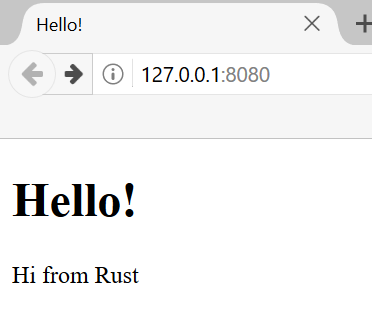
\includegraphics[width=0.7\textwidth]{trpl20-01.png}}
    }
  \caption{Web Server}
  \end{figure}

\column{.45\textwidth}
\begin{itemize}
\item Single-Threated
\item Multithreated
\end{itemize}

\end{columns}

\end{frame}

\section{References}

\begin{frame}
\frametitle{References}
\begin{itemize}
\item History and adoption\\
\href{https://en.wikipedia.org/wiki/Rust_(programming_language)}{https://en.wikipedia.org}
\item Features\\
\href{https://www.rust-lang.org/}{https://www.rust-lang.org}\\
\href{https://www.youtube.com/watch?v=IDpe6k_IIfU}{https://www.youtube.com}\\
\href{https://crates.io/}{https://crates.io}\\
\item Why scientists are turning to Rust\\
\href{https://www.nature.com/articles/d41586-020-03382-2}{https://www.nature.com}
\item Dropbox adoption\\
\href{https://dropbox.tech/infrastructure/rewriting-the-heart-of-our-sync-engine}{https://dropbox.tech}
\item Demo web server\\
\href{https://doc.rust-lang.org/stable/book/ch20-00-final-project-a-web-server.html}{https://doc.rust-lang.org}
\item Presentation and code\\
\href{https://github.com/CarlosAMolina/workshop-rust-web-server}{https://github.com/CarlosAMolina/workshop-rust-web-server}
\end{itemize}
\end{frame}

\begin{frame}
\frametitle{References. Images}
\begin{itemize}
\item Rust logo\\
\href{https://foundation.rust-lang.org/policies/logo-policy-and-media-guide/\#the-rust-trademarks}{https://foundation.rust-lang.org}
\item Ferris the crab, unofficial mascot\\
\href{https://rustacean.net}{https://rustacean.net}
\item Graydon Hoare\\
\href{https://github.com/graydon}{https://github.com/graydon}
\item Rust Foundation founding members\\
\href{https://foundation.rust-lang.org/members/}{https://foundation.rust-lang.org}
\item Multithreaded Web Server\\
\href{https://doc.rust-lang.org/stable/book/ch20-00-final-project-a-web-server.html}{https://doc.rust-lang.org}
\end{itemize}
\end{frame}

\begin{frame}
\Huge{\centerline{Thank you!}}
\end{frame}

\end{document} 
